\documentclass[tikz,border=5pt]{standalone}
\usepackage{amsmath}
\usetikzlibrary{arrows.meta,positioning,calc}

\begin{document}
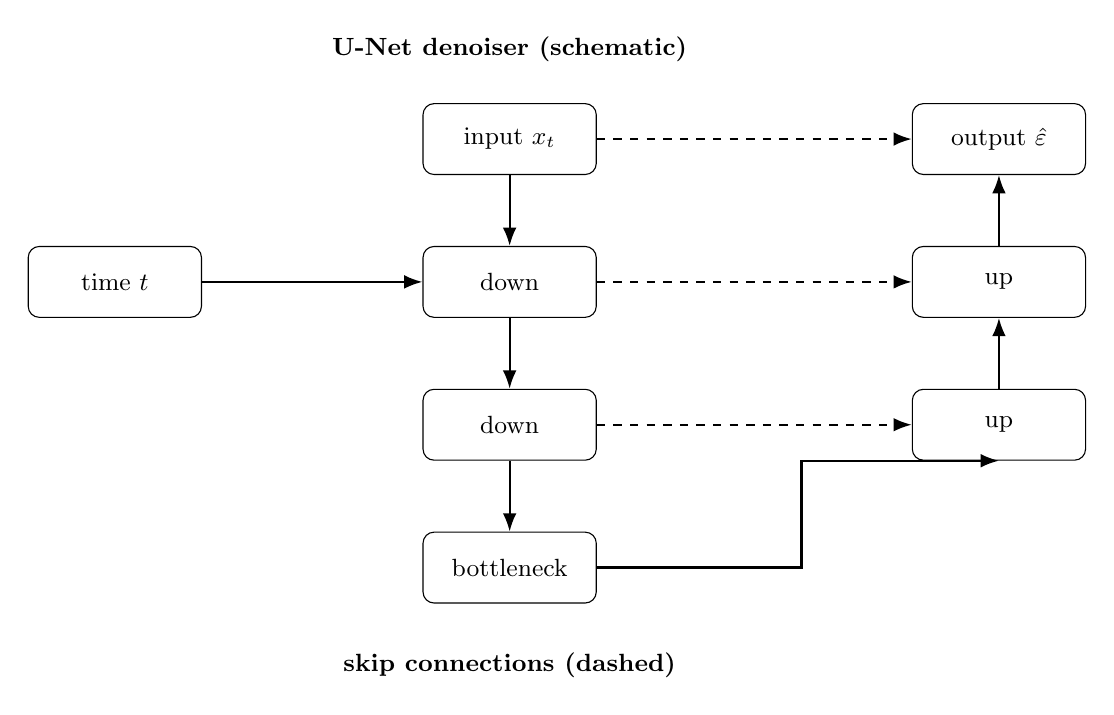
\begin{tikzpicture}[>=Latex, font=\small]
  % encoder blocks (down)
  \node[draw, rounded corners, minimum width=2.2cm, minimum height=0.9cm] (in) {input $x_t$};
  \node[draw, rounded corners, minimum width=2.2cm, minimum height=0.9cm, below=0.9cm of in] (d1) {down};
  \node[draw, rounded corners, minimum width=2.2cm, minimum height=0.9cm, below=0.9cm of d1] (d2) {down};
  \node[draw, rounded corners, minimum width=2.2cm, minimum height=0.9cm, below=0.9cm of d2] (b) {bottleneck};

  % decoder blocks (up)
  \node[draw, rounded corners, minimum width=2.2cm, minimum height=0.9cm, right=4.0cm of d2] (u2) {up};
  \node[draw, rounded corners, minimum width=2.2cm, minimum height=0.9cm, above=0.9cm of u2] (u1) {up};
  \node[draw, rounded corners, minimum width=2.2cm, minimum height=0.9cm, above=0.9cm of u1] (out) {output $\hat\varepsilon$};

  % main flow arrows
  \draw[->, thick] (in) -- (d1);
  \draw[->, thick] (d1) -- (d2);
  \draw[->, thick] (d2) -- (b);
  % route bottleneck -> up without crossing the middle horizontal arrow
  \draw[->, thick] (b.east) -- ++(2.6cm,0) |- (u2.south);
  \draw[->, thick] (u2) -- (u1);
  \draw[->, thick] (u1) -- (out);

  % skip connections
  \draw[->, thick, dashed] (d2.east) -- (u2.west);
  \draw[->, thick, dashed] (d1.east) -- (u1.west);
  \draw[->, thick, dashed] (in.east) -- ++(1.4cm,0) |- (out.west);

  % time embedding arrow
  \node[draw, rounded corners, minimum width=2.2cm, minimum height=0.9cm, left=2.8cm of d1] (t) {time $t$};
  \draw[->, thick] (t) -- (d1.west);

  \node[above=0.4cm of in] {\textbf{U-Net denoiser (schematic)}};
  \node[below=0.5cm of b] {\textbf{skip connections (dashed)}};
\end{tikzpicture}
\end{document}


